\documentclass[%draft,%uncommend to not load any pictures
a4paper,12pt,ngerman,UKenglish,twoside]{book}

%---------------------------------------------------------------------------------------------------------------------------
% Load packages:
%---------------------------------------------------------------------------------------------------------------------------
\usepackage{cmap} % searchable and copyable PDF files in viewer
\usepackage[utf8]{inputenc} % allow to write ä,ö,ü,ß etc
\usepackage[ngerman, UKenglish]{babel} %support German words but have the overall document set up in British English (To write for example by default "List of Figures")
%\renewcaptionname{UKenglish}{\contentsname}{Table of Contents} %uncommend when you want to have a "table of contents" section insteat of just a "contents" section
\usepackage[T1]{fontenc} % suport hyphenation etc.
\usepackage{textcomp} % enabeling \textcelsius (for temperatures) and \textdegree (for latitude, longitude) 
\hyphenation{ja-po-ni-cus Ae-des} % add here some words that dont get hyphenated by default and tend to cause "overfull h-box..."-problems
\usepackage{a4wide} %adjust paper width to European standart A4 paper, otherwise it is american format in LaTex
\usepackage[onehalfspacing]{setspace} % set inline space to 1.5 
\usepackage{emptypage}% don't write page numbers on ampty pages (but cont the pages anyway)
\usepackage[activate={true,nocompatibility},
final,tracking=true,
kerning=true,
spacing=true,
factor=1100,
stretch=10,
shrink=10]{microtype} % optimize block sentence typesetting
\microtypecontext{spacing=nonfrench}
\usepackage{ellipsis} % corrects white space
\usepackage{graphicx} %to insert figure captions
\usepackage[textfont=small, labelfont=small,bf]{caption} % adjust caption format
\usepackage[T1,hyphens]{url} % fix URL-caused badbox problems
\urlstyle{same} % fix URL adresses
\usepackage{etoolbox} % fix URL-caused badbox problems
\apptocmd{\sloppy}{\hbadness 10000\relax}{}{} %minimize amount of badbox problems
\usepackage{afterpage} %dump float figures after calling "\afterpage{\clearpage}"
\usepackage{enumitem} % adjust enumerations
\clubpenalty = 10000 % widow control, 10000 is latex's "worst punishment"
\widowpenalty = 10000 % orphan control, may couse "underfull badboxes", but it looks better like this
\displaywidowpenalty = 10000 % Avoid widows in front of formulas
\vbadness=99999 % hide vbadness problems
\usepackage{pdfpages} % for embedding pdf files
\usepackage{framed}
%\usepackage{listings} % to insert program code
\usepackage{appendix} % Number appendices reasonably

% Math packages:
\usepackage{mathptmx} 
\usepackage{amsmath} 
\usepackage{amssymb} 
\usepackage{amstext} 
\usepackage{nicefrac} % Math package to insert fractions in text

%---------------------------------------------------------------------------------------------------------------------------
% For citing and creating multiple bibliographies (one for each chapter), one needs the package "BibLaTex". 
% Here you can see how to set up BibLaTex:
%---------------------------------------------------------------------------------------------------------------------------

\usepackage{csquotes}
\usepackage{xpatch}
\usepackage[backend=biber, %This is important to set!
bibstyle=numeric-comp, citestyle=chem-acs, 
sortcites=true, 
natbib=true, 
date=year,
hyperref=auto,
maxbibnames=6, minbibnames=6,
giveninits=true, 
terseinits=true, 
isbn=false
]{biblatex}

%---------------------------------------------------------------------------------------------------------------------------
% BibLaTex has some default citation styles. In the following, I customize the "numeric-comp" style to suit the needs in my discipline.
% You may delete this part, stop with the deletion when I say "stop deleting" ;-)
%---------------------------------------------------------------------------------------------------------------------------

\DeclareFieldFormat[article]{titlecase}{\MakeSentenceCase*{#1}} 
\newbibmacro*{journal}{%
  \iffieldundef{journaltitle}
    {}
    {\printtext[journaltitle]{%
       \printfield[myplain]{journaltitle}%
       \setunit{\subtitlepunct}%
       \printfield[myplain]{journalsubtitle}}}}
\DeclareFieldFormat{myplain}{#1}
\DeclareFieldFormat*{title}{#1}
\DeclareFieldFormat{journaltitle}{#1}
  
\DeclareNameAlias{sortname}{last-first}
\DeclareNameAlias{default}{last-first}

\renewcommand*{\multinamedelim}{\addcomma\space}
\renewcommand*{\finalnamedelim}{\addcomma\space}
\renewcommand*{\revsdnamepunct}{}

\renewbibmacro{in:}{%
  \ifentrytype{article}{%
  }{%
    \printtext{\bibstring{in}\intitlepunct}%
  }%
}

\renewbibmacro*{volume+number+eid}{%
  \printfield{volume}%
  \setunit*{\addnbspace}%
  \printfield{number}%
  \setunit{\addcomma\space}%
  \printfield{eid}}
\DeclareFieldFormat[article]{number}{\mkbibparens{#1}}

\renewcommand*{\bibpagespunct}{\addspace}
\DeclareFieldFormat{pages}{#1}

\renewbibmacro*{publisher+location+date}{%
  \printlist{publisher}%
  \setunit*{\addcomma\space}%
  \printlist{location}%
  \setunit*{\addcomma\space}%
  \usebibmacro{date}%
  \newunit}
  
% stop deleting

%---------------------------------------------------------------------------------------------------------------------------
% Insert here one or several files with the bobliographic informations.  In Zotero for example, there is an option for 
% exporting complete BibLaTex bibliographies and also for quickly copying a reference in BibLaTex style.
%---------------------------------------------------------------------------------------------------------------------------
 
\addbibresource{MainDissBib.bib}
\addbibresource{MyBibliography.bib}

%---------------------------------------------------------------------------------------------------------------------------
% More packages:
%---------------------------------------------------------------------------------------------------------------------------

% Equations:
\patchcmd{\subequations}{\def\theequation{\theparentequation\alph{equation}}}
{\def\theequation{\theparentequation.\arabic{equation}}}{}{} % Allow for sub-equations and give them arabic numbers

% Add a list of equations:
\usepackage[nottoc,numbib]{tocbibind}
\usepackage{tocloft}
\newcommand{\listequationsname}{List of Equations}
\newlistof{myequations}{equ}{\listequationsname}
\newcommand{\myequations}[1]{%
\addcontentsline{equ}{myequations}{\protect\numberline{\theequation}#1}\par}
\xpretocmd{\listofmyequations}{\addcontentsline{toc}{chapter}{\listequationsname}}{}{}
\setlength{\cftmyequationsnumwidth}{2.3em}
\setlength{\cftmyequationsindent}{1.5em}

%Tables:
\usepackage{booktabs} 
\usepackage{tabularx}
\usepackage{ltablex} 
\usepackage{longtable}
\usepackage{multicol}
\usepackage{multirow}
\newcolumntype{L}[1]{>{\raggedright\arraybackslash}p{#1}}	% linksbündig mit Breitenangabe
\newcolumntype{C}[1]{>{\centering\arraybackslash}p{#1}} 	% zentriert mit Breitenangabe
\newcolumntype{R}[1]{>{\raggedleft\arraybackslash}p{#1}} % rechtsbündig mit Breitenangabe

% Set bookmarks in the PDF documents (clickable in-document-links and web-links)
\usepackage[bookmarksopen=true,
breaklinks=true,
hidelinks]{hyperref}

% Customizing the header:
\usepackage{fancyhdr} 
\setlength{\headheight}{15pt}
\pagestyle{fancyplain}
\renewcommand{\chaptermark}[1]%
 {\markboth{\thechapter.\ #1}{}}
\renewcommand{\sectionmark}[1]%
 {\markright{\thesection\ #1}}
\lhead[\fancyplain{}{\bfseries\thepage}]%
 {\fancyplain{}{\bfseries\rightmark}}
\rhead[\fancyplain{}{\bfseries\leftmark}]%
 {\fancyplain{}{\bfseries\thepage}}
\cfoot{}

% Format headings:
\usepackage{titlesec}

%---------------------------------------------------------------------------------------------------------------------------
% Set-up of the title page
%---------------------------------------------------------------------------------------------------------------------------
\newcommand{\bigsize}{\fontsize{19.5pt}{25.5pt}\selectfont}
\newcommand{\LMUTitle}{ 
\thispagestyle{empty}
{\parindent0cm
\rule{\linewidth}{.7ex}}
\begin{flushright}
\vspace*{\stretch{1}}
\rmfamily\bfseries\bigsize
The title of the dissertation
\vspace*{\stretch{1}}
\end{flushright}
\rule{\linewidth}{.7ex}

\vspace*{\stretch{3}}
\begin{center}
\begin{large}
Inaugural-Dissertation\\
to obtain the academic degree\\
Doctor rerum naturalium (Dr.\,rer.\,nat.)\\
\vspace*{\stretch{1}}
submitted to the Department of Biology, Chemistry, Pharmacy\\ 
of Freie Universität Berlin\\
\vspace*{\stretch{1}}
by \vspace*{\stretch{1}}
\textsc{My Name}\\
\vspace*{\stretch{2}}
Berlin, 2021
\end{large}
\end{center}
\cleardoublepage
 
\newpage
\thispagestyle{empty}
\begin{flushleft}
Here may stand some information on the research project and project partners.
\end{flushleft}

\vspace*{\stretch{0.1}}
\begin{flushleft}
\begin{large}
First Reviewer: Prof. Dr. Name Surname \\
Second Reviewer: Prof. Dr. Name Surname \\
\vspace*{\stretch{0.1}}
Day of defense: \makebox[5cm][c]{\hfill \makebox[5cm][c] {\hrulefill} \hfill} 
\end{large}
\end{flushleft}
}

%---------------------------------------------------------------------------------------------------------------------------
%Beginn des Dokuments 
%---------------------------------------------------------------------------------------------------------------------------
\begin{document}

%Style list of figures, tables and equations:
\preto\figure{%
  \ifnum\value{figure}=0\addtocontents{lof}{{\bfseries Chapter \thechapter\vskip10pt}}\fi
}
\preto\table{%
  \ifnum\value{table}=0\addtocontents{lot}{{\bfseries Chapter \thechapter\vskip10pt}}\fi
}
\preto\equation{%
  \ifnum\value{equation}=0\addtocontents{equ}{{\vskip10pt \bfseries Chapter \thechapter\vskip10pt}}\fi
}
\captionsetup[figure]{list=no}
 \frontmatter %declaration makes the pages numbered in lowercase roman, and makes chapters not numbered, although each chapter’s title appears in the table of contents; if you use other sectioning commands here, use the *-version.
\LMUTitle
\captionsetup[figure]{list=yes}

\tableofcontents
\markboth{Table of contents}{Table of contents}

%---------------------------------------------------------------------------------------------------------------------------
\markboth{Summary}{Summary}
\addcontentsline{toc}{chapter}{\protect Summary}
\chapter*{Summary}
%---------------------------------------------------------------------------------------------------------------------------

Here is the space for a summary in the original language of the document. In most cases, the summary will cover 1 to 2 pages. The command "cleardoublepage'' will ensure that the next chapter starts on a right side of the thesis book and eventually insert a blank side at the left. 

\cleardoublepage

%---------------------------------------------------------------------------------------------------------------------------
%\selectlanguage{ngerman}
\markboth{Zusammenfassung}{Zusammenfassung}
\addcontentsline{toc}{chapter}{\protect Zusammenfassung}
\chapter*{Zusammenfassung}
%---------------------------------------------------------------------------------------------------------------------------

Here one may include a translation of the thesis summary. One may change the language setting of the dokument in this paragraph with "selectlanguage" to allow for optimal hyphenation etc. Again, use "cleardoublepage" to let start the next chapter on a right side, and don't forget to reset the original language of the document.

\cleardoublepage
%\selectlanguage{UKenglish}

\listoffigures
\markboth{List of Figures}{List of Figures}
\clearpage
\listoftables
\markboth{List of Tables}{List of Tables}
\clearpage
\listofmyequations
\markboth{List of Equations}{List of Equations}
\cleardoublepage

%---------------------------------------------------------------------------------------------------------------------------
\markboth{Thesis Outline}{Thesis Outline}
\addcontentsline{toc}{chapter}{\protect Thesis Outline}
\chapter*{Thesis Outline}
%---------------------------------------------------------------------------------------------------------------------------
Here one may define how much chapter the thesis has and how the work is generally structured. Since sometimes individual chapters have relatively long titles (especially if the titles come from a publication and you can't shorten them afterwards), one can set short titles for each chapter that appear in the chapter overview and page headers. I found it convenient to list the short titles briefly here in this section as well, as follows:
\par\bigskip
\begin{flushleft}
\textbf{Chapter 1}\\
General Introduction
\par\medskip
\textbf{Chapter 2}\\
Short title: Short title of Chapter 2\\
Long title: This is a long title of Chapter 2 that does not fit in the page header\\
\par\medskip
\textbf{Chapter 3}\\
Short title: Short title of Chapter 3\\
Long title: This is a long title of Chapter 3 that does not fit in the page header\\
\par\medskip
\textbf{Chapter 4}\\
General Discussion and Conclusions
\end{flushleft}

\cleardoublepage

%---------------------------------------------------------------------------------------------------------------------------
\markboth{List of publications with author contributions}{List of publications with author contributions}
\addcontentsline{toc}{chapter}{\protect List of publications with author contributions}
\chapter*{List of Publications with Author Contributions}
%---------------------------------------------------------------------------------------------------------------------------

\begin{flushleft}
\textbf{Name, My}, Co-Author 1, Co-Author 2. Title \textit{Journal Name} 12, no. 1 (14 March 2019): 106. \url{https://doi.org/10.1186/s13071-019-3368-0.}
\par\medskip
{{MN}} and C1 were responsible for the conception and design of the study. Mn draftred the manuscript. C2 contributed expert knowledge. MN, C1 and C2 critically revised the manuscript. All authors read and approved the final manuscript.
\par\bigskip
\textbf{Name, My}, Co-Author 1, Co-Author 2. Title \textit{Journal Name} 12, no. 1 (14 March 2019): 106. \url{https://doi.org/10.1186/s13071-019-3368-0.}
\par\medskip
MN and C1 were responsible for the conception and design of the study. Mn draftred the manuscript. C2 contributed expert knowledge. MN, C1 and C2 critically revised the manuscript. All authors read and approved the final manuscript.
\end{flushleft}

\cleardoublepage

%%%%%%%%%%%%%%%%  Start Introduction   %%%%%%%%%%%%%%%%%%%%

\mainmatter\setcounter{page}{1} %reset page number
 
 %---------------------------------------------------------------------------------------------------------------------------
\chapter[General Introduction]{General Introduction}
%---------------------------------------------------------------------------------------------------------------------------
\begin{refsection}

Here stands an introduction. In my case, I explained a lot about health risks posed by mosquitoes, especially invasive mosquitoes in Europe. Introductions are always full of citations \cite{kampen_approaches_2015, bartumeus_citizen_2018, caputo_zanzamapp_2020} and subchapters (see e.g. section \ref{sec:example}. Sometimes you may find tables (see e.g. Tab.\ref{Tab:CitizenScience}) and figures (). 

\begin{table}[htb!]
\begin{center}
\caption[Citizen science programmes for studying the mosquito fauna in Europe]{Citizen science programmes for studying the mosquito fauna in Europe  \cite{kampen_approaches_2015, bartumeus_citizen_2018, caputo_zanzamapp_2020}}
\begin{small}
\begin{tabular}{lll}
\toprule
Country & Name & Submissions \\ 
\toprule
France & iMoustique & photograph via smart-phone application\\ 
Germany & Mückenatlas & physically via mail \\ 
Italy & ZanzaMapp & online questionnaire\\
Portugal & MosquitoWEB & physically via mail \\ 
Spain & Mosquito Alert & photograph via smart-phone application\\ 
& (former “Atrapa el Tigre”) &\\
The Netherlands & Muggenradar & physically via mail \\ 
UK & Mosquito Reporting Scheme & physically via mail \\ 
\bottomrule
\end{tabular} 
\end{small}
\label{Tab:CitizenScience}
\end{center}
\end{table}

\begin{figure}[!htb]
\centering
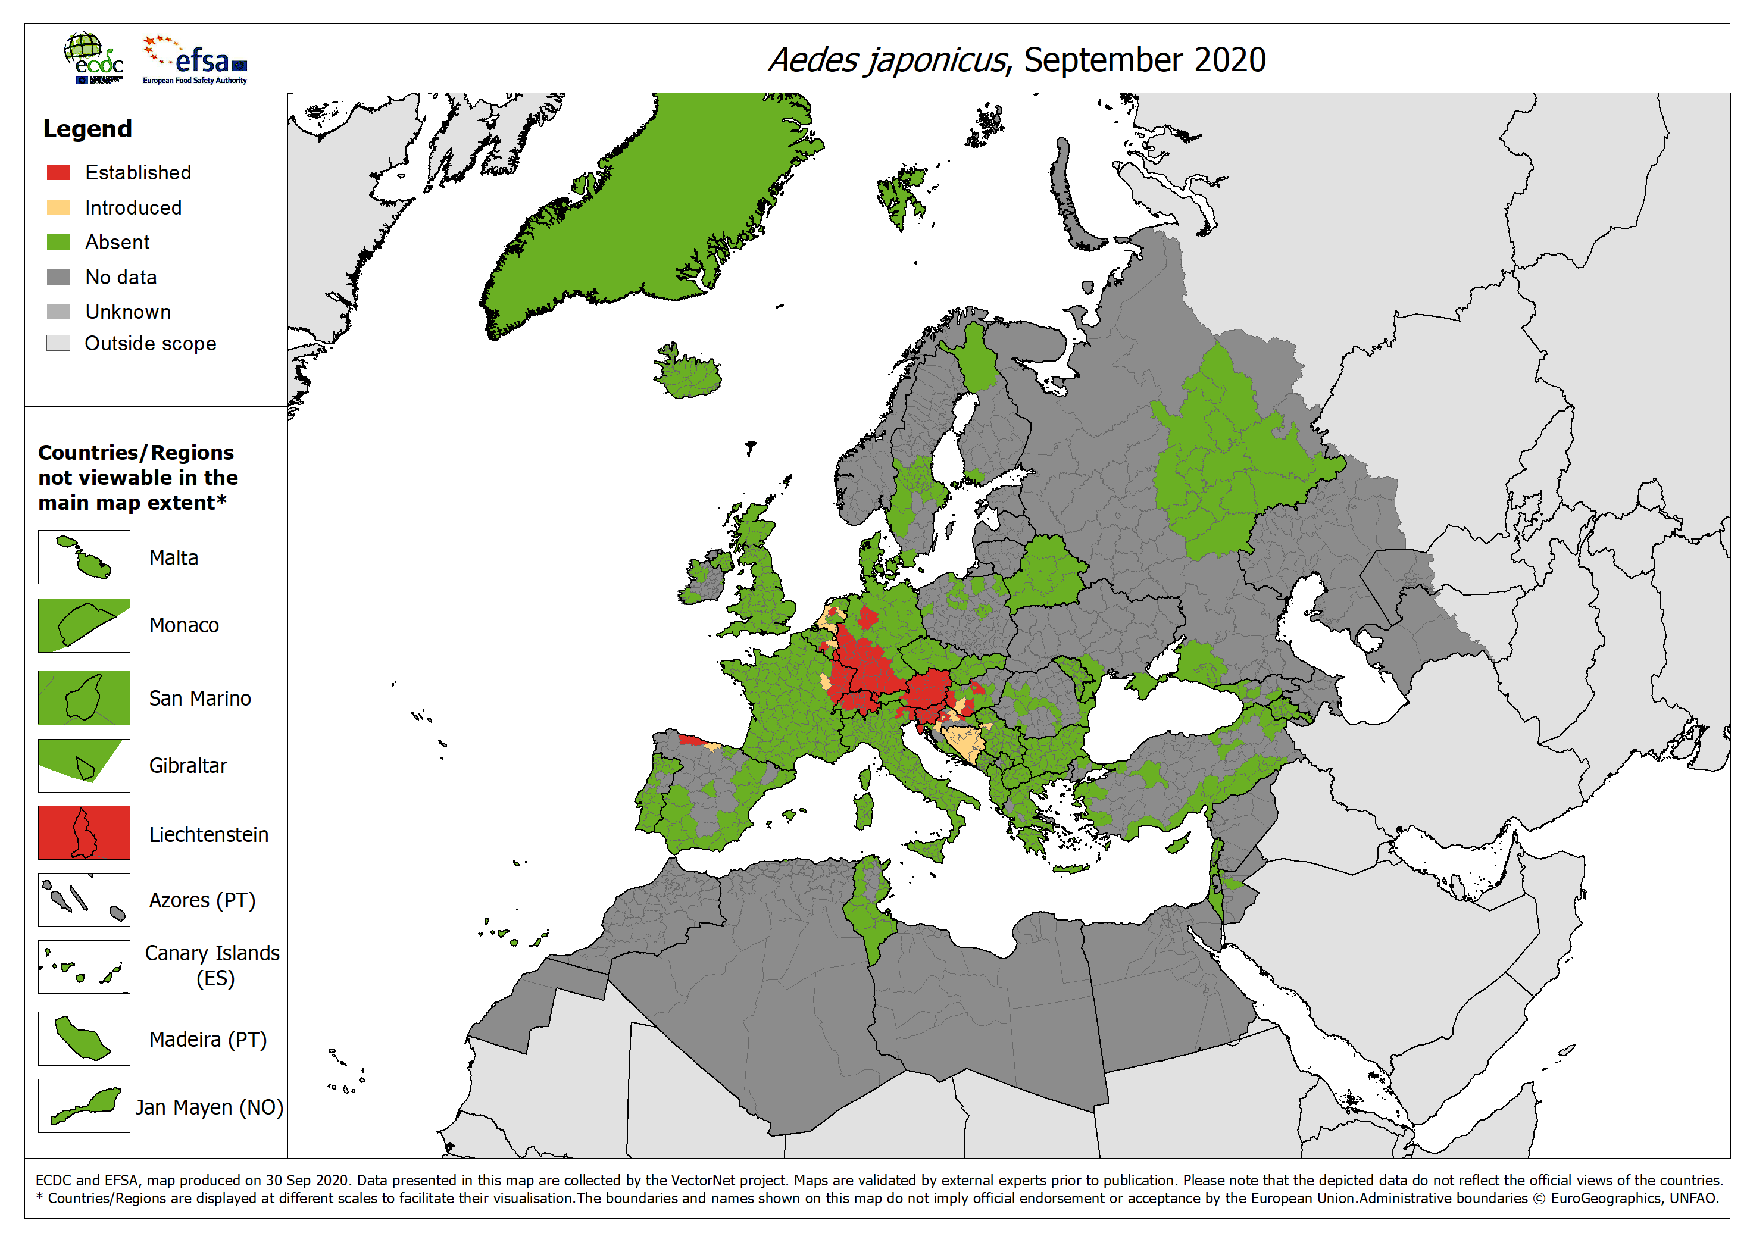
\includegraphics[width=\textwidth]{Intro_AedesJaponicusMap.pdf}
\caption[Current known distribution of \textit{Aedes japonicus japonicus} in Europe at the 30th of September 2020]{Current known distribution of \textit{Aedes japonicus japonicus} in Europe at the 30th of September 2020 \cite{ecdc_aedes_2020}.}
\label{fig:IntroJaponicusDistribution}
\end{figure}

Generally, in the LaTex book class, the sections hierarchie is: chapter, section, subsection, subsubsection, paragraph and finally subparagraph:

%\chapter[Example short chapter title]{example chapter title}
\section[Example short section title]{Example section title}\label{sec:example}
\subsection[Example short subsection title]{Example subsection title}
\subsubsection[Example short subsubsection title]{Example subsubsection title}
\paragraph{Example paragraph title}
%\subparagraph{Example subparagraph title}

\section{Research questions}
In summary, the leading questions of my work were:
\begin{enumerate}[label=(\roman*)]
\item Leading question 1
\item Leading question 2
\end{enumerate}

\section{References}
\printbibliography[heading=none]
\end{refsection}

%---------------------------------------------------------------------------------------------------------------------------
\chapter{Short title of Chapter 2}
%---------------------------------------------------------------------------------------------------------------------------
\begin{refsection}

{\Large This is a long title of Chapter 2 that does not fit in the page header}

\paragraph[Authors]{Authors}
My Name$^{ a, b}$, Co-Author 1$^{ a}$, Co-Author 2$^{ c}$
\vskip1em
\begin{footnotesize}
\begin{enumerate}[nosep,leftmargin=*,font=\itshape]
\item[a] Adress first institution
\item[b] Adress second institution
\item[c] Adress third institution
\end{enumerate}
\end{footnotesize}

\paragraph[Keywords]{Keywords}
Keyword 1, Keyword 2, Keyword 3, Keyword 4

\paragraph[Journal]{Journal}
Parasitology Research (Springer Nature), published in print in issue 119:31--42 (2020). \url{https://doi.org/10.1007/s00436-019-06513-5}

\clearpage

\section[Abstract]{Abstract}
Here stands the abstract.

\section[Introduction]{Introduction}
Here is the introduction of Chapter 2. The introduction is full of references \cite{medlock_entomological_2015, becker_mosquitoes_2014}.

\section[Materials and methods]{Materials and methods}
Here, the methodology is explained in detail. Sometimes, it is necessary to include equations. I set up an overview of the equations after the ``List of Figures'' caption (see \ref{Eq:Chap2_a} and \ref{Eq:Chap2_b}).
 
\begin{equation}
A = \frac{B}{C}
\label{Eq:Chap2_a}
\end{equation}\myequations{Title of an example equation}

\begin{equation}
E = mC^{2}
\label{Eq:Chap2_b}
\end{equation}\myequations{Title of another example equation}


\section[Results]{Results}
Here will stand the results. They may include lots of figures and tables.

\section[Discussion]{Discussion}
A discussion chapter usually has a lot of references \cite{kerkow_what_2019, koban_asian_2019}.

\section[Conclusions]{Conclusions}
Our model approach appears to be suitable for ...

\paragraph*{Acknowledgements}
We thank two anonymous reviewers for their helpful comments on the manuscript.

\paragraph*{Funding information}
This paper was funded by ...

\paragraph*{Data availability}
Explanation of the data availability.

\subsubsection*{Compliance with ethical standards}
\paragraph*{Conflict of interest}
The authors declare that they have no conflict of interest.

\paragraph*{Open Access}
 This article is distributed under the terms of the Creative Commons Attribution 4.0 International License (\url{http://creativecommons.org/licenses/by/4.0/})...

\section[References]{References}
\printbibliography[heading=none]
\end{refsection}

%---------------------------------------------------------------------------------------------------------------------------
\chapter{Short title of Chapter 3}
%---------------------------------------------------------------------------------------------------------------------------
\begin{refsection}
{\Large This is a long title of Chapter 3 that does not fit in the page header}

\paragraph[Authors]{Authors}
My Name$^{ a, b}$, Co-Author 1$^{ a}$, Co-Author 2$^{ c}$
\vskip1em
\begin{footnotesize}
\begin{enumerate}[nosep,leftmargin=*,font=\itshape]
\item[a] Adress first institution
\item[b] Adress second institution
\item[c] Adress third institution
\end{enumerate}
\end{footnotesize}

\paragraph[Keywords]{Keywords}
Keyword 1, Keyword 2, Keyword 3, Keyword 4

\paragraph[Journal]{Journal}
Submitted to Ecological Modelling (Elsevier) on 12 March 2021 in an abbreviated form.

\clearpage

\section[Abstract]{Abstract}
Here stands the abstract.

\section{Introduction}
\subsection{Background}
Here is a text full of references \cite{chancey_global_2015, gray_review_2014}.


\subsubsection{Objectives}
Here is more text with more citations \cite{yaremych_west_2004, deoya_high_2018}.

\subsection{Summary of model innovations} 
Our work presents the following innovations to existing models: 
\begin{enumerate}[label=(\roman*)]
\item innovation 1
\item  innovation 2
\end{enumerate}

\section{Materials and Methods}
\subsection{Study regions}\label{Chap:StudyRegions}
We selected three subregions of the grid based habitat suitability map with sizes of 25\,km $\times$ 25\,km for model applications (Fig.\,\ref{fig:RegionsInGermany}). In each of them, the occurrence of \textit{Ae.\,j.\,japonicus} has been documented for several years \cite{werner_further_2013, walther_citizen_2017}.

\begin{figure}[htb]
\centering
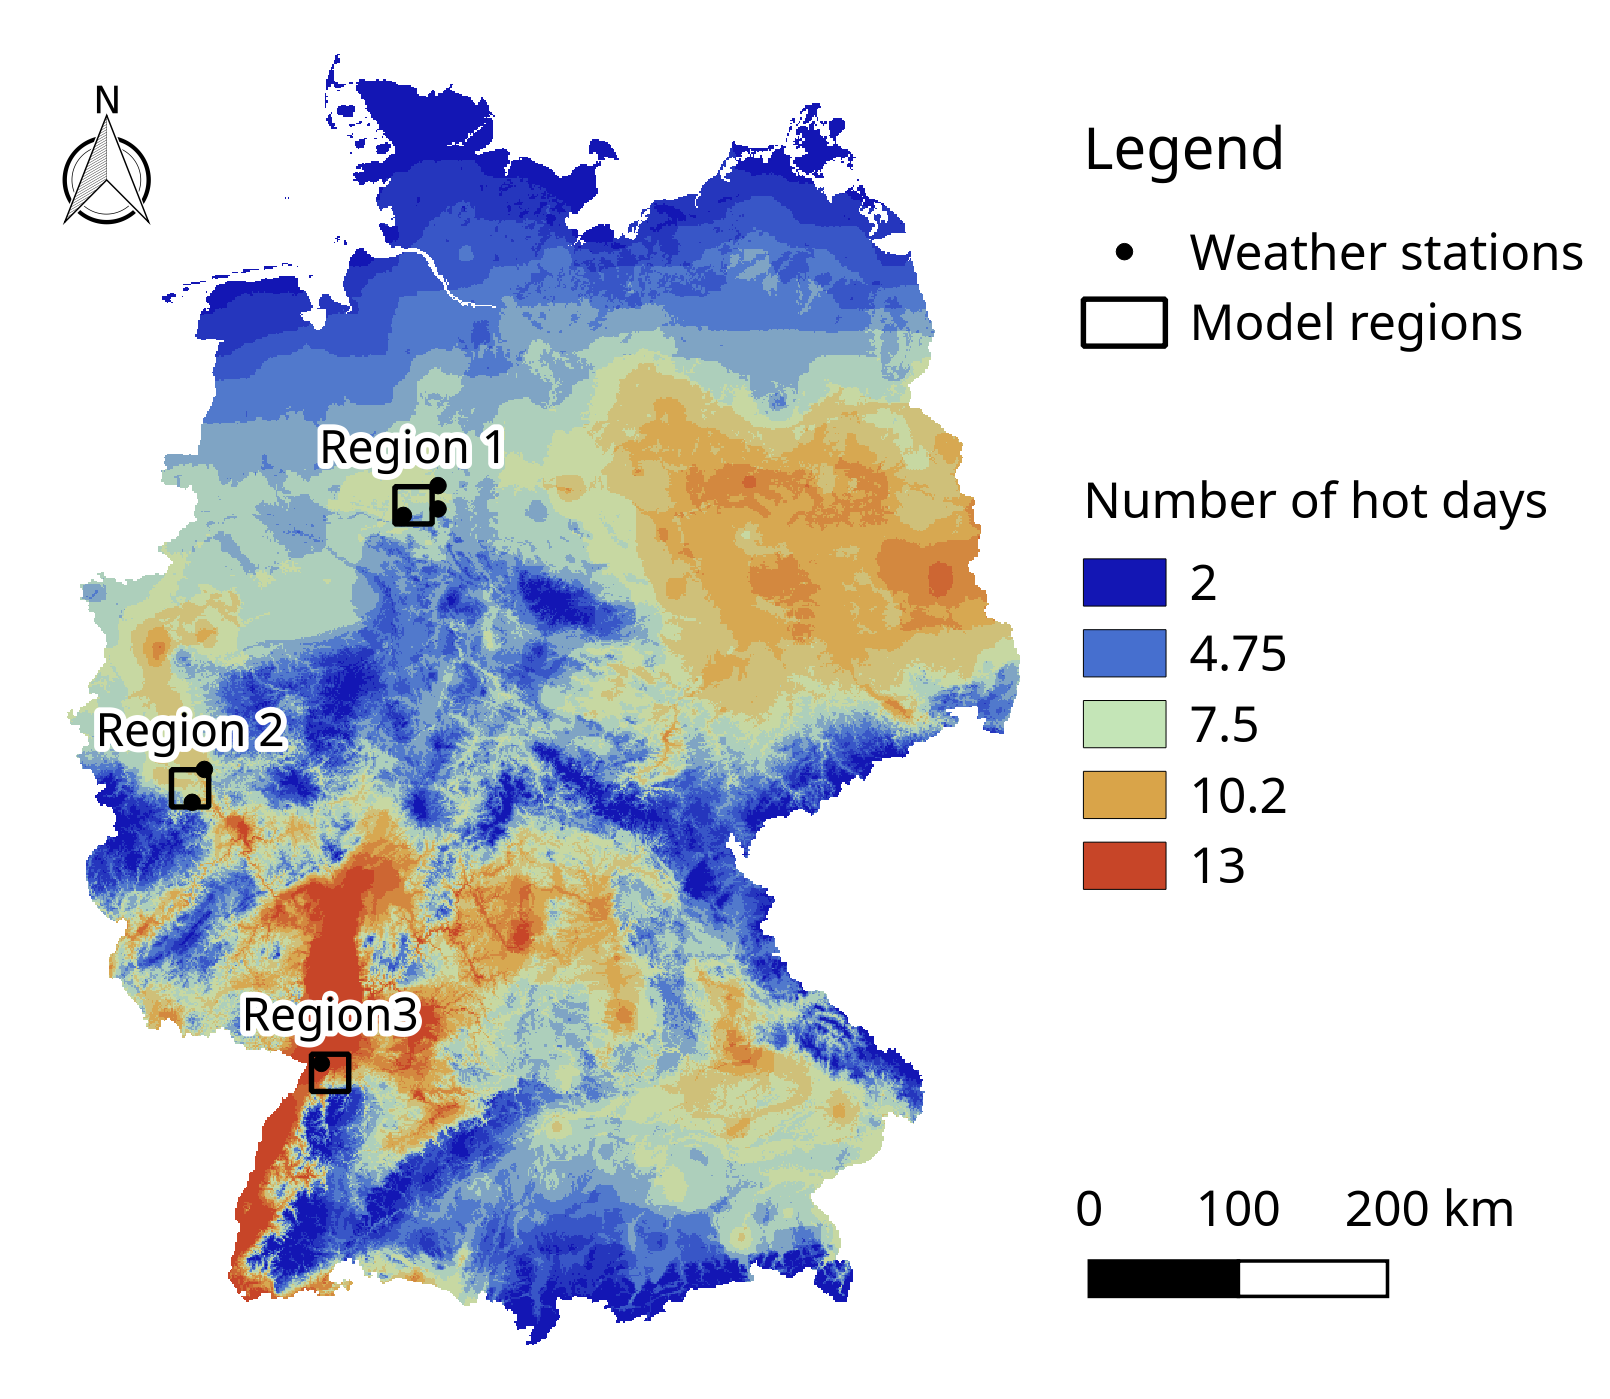
\includegraphics[width=0.65\textwidth]{WNV_Map.png}
\caption[Location of the study regions, their nearest weather stations, and illustration of the number of local hot days]{Location of the study regions, their nearest weather stations, and illustration of the number of local hot days defined by a maximum air temperature higher than 30\textcelsius{} (annual mean of the long-term period 1981-2010). Geodata source: German Weather Service.}
\label{fig:RegionsInGermany} 
\end{figure}

\subsection{Calculation of the day length}
For the calculation of the day lengths, we apply the Brock model \cite{brock_calculating_1981} which maps the latitude ($l$) of the location and the day ($d$) of the year on the day length as follows:
%
\begin{equation}
D(l,d) = 2 \tfrac{cos^{-1}\left( -tan(l) tan\left( 23.45 sin \left(360 \tfrac{283+d}{365}\right) \right) \right)}{15}
\label{eq:Daylength}
\end{equation}\myequations{Daylength}

\subsection{Sub-models}
\subsubsection{Time component}
The model is based on 9 compartments (ordinary differential equations) that describe the populations and infection stages of mosquitoes and birds by means of a density-dependent approach (equations \ref{eq:LM}-\ref{eq:DB}). The mosquito compartments include larvae ($L_{M}$), susceptible  ($S_{M}$), exposed ($E_{M}$) and infectious mosquitoes ($I_{M}$). The bird compartments are susceptible ($S_{B}$), exposed ($E_{B}$), infectious ($I_{B}$), recovered ($R_{B}$) and dead birds ($R_{B}$). Recovered birds have always acquired immunity and the dead birds refer only to those that have succumbed to WNV. 

The equations are taken from previous compartment models for Usutu virus and WNV \cite{rubel_explaining_2008, laperriere_simulation_2011}, but we introduced a species specific probability of the mosquitoes taking a blood meal on a bird and an additional probability of taking blood meals on a host bird when feeding on a bird. Both factors affect the virus transmission rates. We have also changed parameters that describe the characteristics of host birds and vector mosquitoes. All fix parameters of the differential equations are summarised in table \ref{Tab:FixParams}.

\subparagraph{Mosquito compartments}
\begin{subequations}
\begin{align}
\frac{d L_{M}}{dt} &= (b_{L}(T)\delta_{M}(D)N_{M} - m_{M}(T)L_{M}) \left( 1- \frac{L_{M}}{K_{M}}\right) - b_{M}(T) L_{M}\label{eq:LM}\\ \addlinespace
\frac{d S_{M}}{dt} &=b_{M}(T) L_{M} - m_{M}(T) S_{M} - \lambda_{BM}(T,D) S_{M}\label{eq:SM}\\ \addlinespace
\frac{d E_{M}}{dt} &= \lambda_{BM}(T,D) S_{M} - \gamma M(T) E_{M} - m_{M}(T) E_{M}\label{eq:EM}\\ \addlinespace
\frac{d I_{M}}{dt} &= \gamma M(T) E_{M} - m_{M}(T) I_{M}\label{eq:IM}
\end{align}
\end{subequations}\myequations{Differential equations for the life and infection stages of the vector mosquitoes}

\subparagraph{Bird compartments}
\begin{subequations}
\begin{align}
\frac{d S_{B}}{dt} &= \left(b_{B}-(b_{B}-m_{B}) \frac{N_{B}}{K_{B}}\right) N_{B}-\lambda_{MB}(T,D)  S_{B} - m_{B} S_{B}\label{eq:SB}\\ \addlinespace
\frac{d E_{B}}{dt} &= \lambda_{MB}(T,D) S_{B} - \gamma_{B} E_{B} - m_{B} E_{B}\label{eq:EB}\\ \addlinespace
\frac{d I_{B}}{dt} &= \gamma_{B} E_{B} - \alpha_{B} I_{B} - m_{B} I_{B}\label{eq:IB}\\ \addlinespace
\frac{d R_{B}}{dt} &= (1 - \nu_{B}) \alpha_{B} I_{B} - m_{B} R_{B}\label{eq:RB}\\ \addlinespace
\frac{d D_{B}}{dt} &= \nu_{B} \alpha_{B} I_{B}\label{eq:DB}
\end{align}
\end{subequations}\myequations{Differential equations for the infection stages of the host birds}
% \pagebreak

\begin{table}[!htb]
\begin{center}
\caption{State variables}
\begin{small}
\begin{tabular}{ p{1cm}  p{10cm}  p{2.5cm}}
\toprule
Term & Description & Value\\ 
\toprule
$ m_{B} $ &  Average mortality rate of magpies & 0.001404\,d$^{-1}$ \\
$ \gamma_{B} $ &  Rate infected--infectious magpies & 0.333\,d$^{-1}$ \\
$ \nu_{B} $ &  Portion of magpies dying due to WNV infection & 0.43 \\
$ p_{M} $ &  Transmission efficiency from infectious mosquito to bird & 1.0 \\
$ \alpha_{B} $ &  Removal rate of magpies due to WNV infection & 0.28\,d$^{-1}$ \\
\midrule
$ p_{B_{J}} $ & Transmission efficiency from infectious bird to \textit{Ae.\,j.\,japonicus} & 0.17 \\
$ p_{B_{C}} $ &  Transmission efficiency from infectious bird to \textit{Culex agg.} & 0.06 \\
$ P_{J} $ &  Proportion of \textit{Ae.\,j.\,japonicus} blood meals taken on birds  & 0.18 \\
$ P_{C} $ &  Proportion of \textit{Culex agg.}~blood meals taken on birds  & 0.33, 0.66, 0.96 \\
\bottomrule
\end{tabular} 
\end{small}
\label{Tab:FixParams}
\end{center}
\end{table}

\section{Results}
Here the results are presented.

\section{Discussion}
Here will be the discussion.

\section{Conclusions}
...

\section[References]{References}
\printbibliography[heading=none]
\end{refsection}

%---------------------------------------------------------------------------------------------------------------------------
% Here you find a way of how to include PDF pages as a separate chapter 
% (e.g. if one wants to include published articles directly:
%---------------------------------------------------------------------------------------------------------------------------

%\includepdf[pages=-,
%pagecommand={\phantomsection\addcontentsline{toc}{section}{test}},
%frame= false,
%width=1.2\textwidth,
%offset= 0mm -15mm
%]{Fuzzypaper.pdf}

%---------------------------------------------------------------------------------------------------------------------------
\chapter{General Discussion and Conclusions}
%---------------------------------------------------------------------------------------------------------------------------
\begin{refsection}

At the end of the work, the findings are put into a broader context and the significance of the outcomes is discussed. The results should be compared with those of previous studies \cite{wieland_automated_2017, fruh_modelling_2018}. 

\section[References]{References}
\printbibliography[heading=none]
\end{refsection}

%\backmatter %leaves the page numbering alone but switches the chapters back to being not numbered.
%\refstepcounter{chapter}
\begin{appendices}

%---------------------------------------------------------------------------------------------------------------------------
\addcontentsline{toc}{chapter}{\protect Appendices}
\chapter*{Appendices}
%---------------------------------------------------------------------------------------------------------------------------

%\addcontentsline{toc}{chapter}{\protect Statement of Academic Integrity}
\chapter{Statement of Academic Integrity}
I hereby declare that I have written the dissertation presented here independently and so on... Check the website of your university department for standardized texts!

%\addcontentsline{toc}{chapter}{\protect Acknowledgements}
\chapter{Acknowledgements}
Here is the place to acknowledge the supervisors, family, friends and so on.

\end{appendices}
\end{document}
